\chapter{Tehnologije}\label{ch:tehnologije}

U ovom poglavlju će biti opisane tehnologije korišćene za razvoj rešenja.

\section{React}\label{sec:react}
\textit{React} je \textit{Javascript} biblioteka za građenje korisničkog interfejsa. Koristi se za kreiranje modernih 
reaktivnih korisničkih interfejsa koji se mogu izgraditi uz pomoć izolovanih delova koda. Ti delovi koda nazivaju 
se komponente. Korišćenjem komponente omogućeno je deljenje aplikacije na nezavisne delove koji se prilikom razvoja 
mogu iznova koristiti.~\cite{react}

Svaka komponenta sastoji se iz metode za renderovanje i sadrži podatke o tome šta je sve potrebno da se prikaže 
krajnjem korisniku. Mogu biti klasne ili funkcijske. Funkcijske komponente kao ulazni parametar primaju svojstva 
i vraćaju \textit{JSX} element. Sa druge strane, klasne komponente su definisane kao \textit{ES6} 
klase i renderuju \textit{React} elemente koristeći \texttt{render()} metodu. 

Kako bi komunicirale međusobno sa ostalim delovima aplikacije, komponente moraju imati svoje stanje (engl. \textit{state}) 
i svojstva (eng. \textit{properties - props}). Svojstva i stanje predstavljaju čist \textit{JavaScript} objekat. Izmena bilo kojeg 
od ova dva objekta okida ponovno renderovanje komponente. 

Svojstva čine \textit{React} komponente fleksibilnim i pogodnim za 
ponovno korišćenje. Prosleđivanjem različitih svojstava, komponente se mogu ponašati i izgledati drugačije. Svojstva komponente 
služe isključivo za prikaz i unutar same komponente ih ne bi trebalo menjati. Protok informacija mora biti jednosmeran od višeg 
nivoa komponente ka nižem. Stoga je komponenta sa višeg nivoa zadužena za prosleđivanje skupa svojstava.

Stanje komponente se koristi za “pamćenje” podataka unutar same komponente. Možemo reći da je stanje privatno, jer se stanju 
komponente ne može pristupiti iz roditeljske komponente. Može se promeniti na osnovu korisnikove interakcije ili neke druge 
akcije unutar aplikacije. Za razliku od svojstava, stanjem se može upravljati unutar same komponente.

\textit{React} kuke (eng. \textit{hooks}) služe za korišćenje stanja u funkcijskim komponentama. U teoriji, kuke su funkcije 
koje se “kače” za stanja i životne cikluse unutar funkcijske komponente. Da bi se koristile \textit{React} kuke, moraju se 
poštovati dva pravila:
\begin{itemize}
    \item Pozivanje kuka se mora vršiti sa najvišeg nivoa. To znači da se one ne smeju pozivati unutar petlji, 
    postavljenih uslova ili ugnježdenih funkcija.
    \item Pozivanje kuka se ne može vršiti iz običnih \textit{JavaScript} funkcija, već samo iz funkcija \textit{React} komponente.
\end{itemize}

Stanje svake komponente je potpuno nezavisno. Korišćenjem kuka, postiže se to da se logika sa stanjem može ponovo koristiti 
(ali ne i samo stanje). Ustvari, svakim pozivom kuke dobijamo potpuno izlovano stanje, pa se stoga jedna kuka može koristiti 
više puta unutar jedne komponente. Pored toga, kuke omogućavaju pravljenje kompozicije. Unutar jedne kuke je moguće zakačiti 
drugu kuku i tako napraviti kompoziciju. 

Pre uvođenja kuka, u \textit{React}-u se koristio obrazac zvan “komponente višeg reda” (eng. \textit{Higher-Order Components}). 
Konkretno, komponenta višeg reda je funkcija koja za argument prihvata komponentu i vraća novu komponentu. Kako su i ulaz i 
izlaz istog tipa (\textit{React} komponenta), lako se može zaključiti da se komponente višeg reda mogu komponovati, a logika i 
stanje koje one dodaju se mogu iskoristiti na više različitih mesta. Iako je i dalje moguće koristiti ovaj obrazac, jer je 
nezavisan od toga da li je komponenta napisana kao klasa ili kako funkcija, preporučuje se koršćenje kuka, kad god je moguće. 
Naime, kuke imaju dve glavne osobine koje imaju i komponente višeg reda: ponovno korišćenje i kompoziciju. Glavna prednost kuka 
u odnosu na komponente višeg reda je to što su zavisnosti eksplicitne kod kuka. Sa druge strane, kuke se mogu koristiti samo u 
funkcijskim komponentama pa je upotreba komponenti višeg reda opširnija.

Glavna prednost \textit{React} kuka je enkapsulacija. Odgovornost za prikazivanje korisničkog interfejsa ostaje na samoj 
komponenti, a logika prikaza za tu komponentu se prebacuje u kuku koja se vezuje za tu komponentu. Na taj način se štiti 
od neželjenog pristupa unutrašnjim podacima od strane komponente i sakriva se kompleksnost. Uz sve navedeno, 
testiranje postaje lakše jer se odvojeno mogu testirati prikaz korisničkog %TODO interfejsa od logike
interfejsa od logike prikaza. 

Prilikom razvoja aplikacije susrećemo se sa izazovima kao što je kreiranje konzistentnih komponenti koje izgledaju i funkcionišu 
na isti način, ne samo unutar jedne aplikacije već i na mnogim drugim aplikacijama koje se razvijaju. Ispis identičnih stilova 
komponenata iznova i izmena promenljivih vrednosti na više mesta u aplikaciji utiče na vreme razvoja aplikacije.

Umesto da se stilovi koriste globalno, teži se ka tome da se postave standardizovane komponente sa ugrađenim funkcionalnostima i 
stilovima kako bi se one mogle koristiti iznova i podešavati jednostavno u zavisnosti od slučaja u kojem se koriste.
Jedna od popularnijih biblioteka za stilizovanje \textit{React} komponenata je \textit{Material-UI}. Ona predstavlja 
implementaciju \textit{Google}-ovog \textit{Material Design}-a. Uz pomoć ove biblioteke komponente se mogu koristiti zasebno, 
koristeći samo one stilove koji treba da budu prikazani.

\textit{Material UI} biblioteka koristi \textit{CSS} u \textit{JS} (eng. \textit{CSS-in-JS}). Korišćenjem globalnih \textit{CSS} 
fajlova, a zbog kaskadne prirode \textit{CSS}-a (\textit{Cascading Style Sheets}), stilovi se mogu učitati u bilo kom redosledu 
i pregaziti neki drugi stil. Pisanjem \textit{CSS} u \textit{JavaScript}-u rešava problem zavisnosti jer se mogu koristiti 
\textit{JavaScript} moduli. Na taj način se komponente mogu pokretati nezavisno, bez oslanjanja na eksterne \textit{CSS} fajlove. 
Kako danas većina alata za izgradnju projekta podržava pronalaženje i brisanje koda koji se ne koristi, a samim tim i smanjuju 
veličinu izgrađenog projekta, ova tehnika se može primeniti i na \textit{CSS} u \textit{JS}. Stilovi su opisani preko 
\textit{JavaScript} objekata i kao takvi mogu da pristupe stanju komponente što povećava fleksibilnost pisanja samih stilova.


\section{NestJS}\label{sec:nestjs}
Razvoj aplikacije na \textit{Node.js} platformi vremenom može postati kompleksan. Što se više svojstava 
dodaje u aplikaciju, to baza koda postaje sve veća.

\textit{NestJS} je radni okvir za građenje efikasne, skalabilne \textit{Node.js} aplikacije na serveru. 
Pruža serverskom delu aplikacije modularnu strukturu za organizaciju koda u odvojene module i služi 
za eliminisanje neorganizovane baze kodova.

Korišćenjem \textit{NestJS} programerima se pruža mogućnost da koriste sve benefite JavaScript-a i uz
to pišu kod za klijentski i serverski deo aplikacije u istom programskom jeziku. Sadrži komponente 
funkcionalnog, objektno orijentisanog i funkcionalno reaktivnog programiranja.

Inspirisan \textit{Angular}-om, \textit{NestJS} je napisan u programskom jeziku \textit{TypeScript} 
i koristi \textit{Express.js}, koji ga čini kompatibilnim sa većinom \textit{Express} posredničnih 
(eng. \textit{middleware}) softvera. Za razvoj podržava JavaScript i TypeScript, kao i PostgreSQL, 
MongoDB i MySQL baze podataka.

Osnovne gradivne komponente NestJS aplikacije su kontroleri, provajderi i moduli.

Kao i kod većine radnih okvira, kontroleri u \textit{NestJS} su odgovorini za upravljanje %TODO dolaznih zahteva
svih dolaznih zahteva i povratnih odgovora ka klijentskom delu aplikacije. \textit{NestJS} je struktuiran tako da je 
mehanizam za usmeravanje, prikazan na slici \ref{fig:kontroler} sposoban da kontroliše koji kontroler 
će biti zadužen za određeni zahtev.
Kako bi se napravio osnovni kontroler, koriste se klase i dekoratori. Dekoratori pridruzuju meta 
podatke klasama i omogućavaju \textit{Nest}-u da kreira mapu za rutiranje. Za definisanje HTTP 
metoda za rute, koriste se dekoratori \texttt{@Get()}, \texttt{@Put()}, \texttt{@Post()} i \texttt{@Delete()}.~\cite{nest}

\begin{figure}[h]
    \centering
    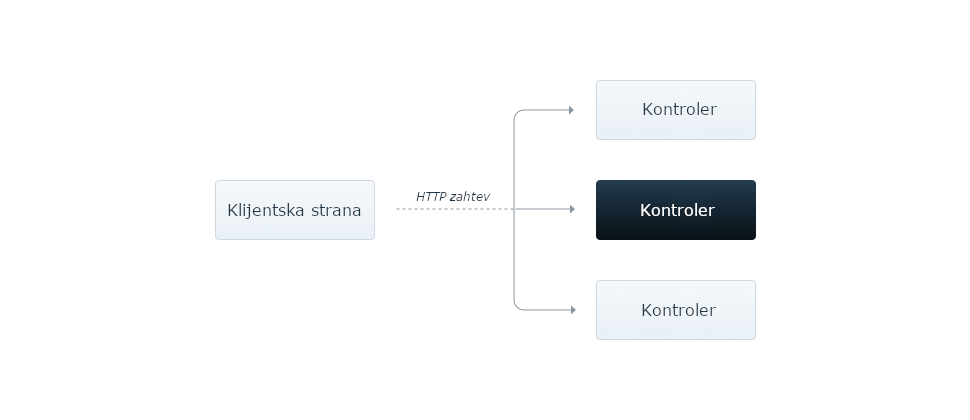
\includegraphics[width=1\textwidth]{kontroler}
    \caption{Usmeravanje zahteva}
    \label{fig:kontroler}
\end{figure}
  
\textit{Nest} provajderi se mogu umetnuti u kontrolere ili u druge provajdere. Nazivaju se i servisi, 
i dizajnirani su da apstrahuju bilo koji oblik složenosti i logike.
Servisni provajder u \textit{Nest} je klasa sa specijalnim dekoratorm \texttt{@Injectable()}. 

Moduli omogućavaju grupisanje povezanih fajlova. To su TypeScript fajlovi dekorisani sa 
\texttt{@Module} dekoratorom, koji pruža meta podatke koje \textit{Nest} koristi za organizaciju 
strukture aplikacije. Svaka \textit{Nest} aplikacija mora imati bar jedan modul - osnovni modul. 
Preporučuje se da se velike aplikacije rastave na više modula kako bi se lakše kontrolisala 
struktura aplikacije.

Tri osnovna koncepta NestJS su:
\begin{itemize}
\item \textbf{DTO}: Objekat za prenos podataka (eng. \textit{Data transfer object}) je objekat 
koji definiše kako će se podaci poslati preko mreže
\item \textbf{Interfejsi} : \textit{TypeScript} interfejsi se koriste za proveru tipa i 
definisanje tipova podataka koji se mogu proslediti kontroleru ili \textit{NestJS} servisu
\item \textbf{Umetanje zavisnosti}: (eng. \textit{Dependency Injection}) je obrazac projektovanja 
koji se koristi za povećanje efikasnosti i modularnosti aplikaicje. Održava kod čistim i 
lakšim za korišćenje. U \textit{NestJS} se koristi za pravljenje uvezanih komponenata.~\cite{nest_getting_started}
\end{itemize}

\section{GitHub aplikacija}\label{sec:github_app}
Aplikacije na \textit{GitHub}-u mogu automatizovati i poboljšati tok razvoja. \textit{GitHub} 
aplikacije se preporučuju za integrisanje sa \textit{GitHub}-om jer nude granularnije permisije 
za pristup podacima. Rade samostalno, preduzimajući akcije putem \textit{API}-ja, koristeći 
sopstveni identitet. 

\textit{GitHub} aplikacije se mogu instalirati direktno na organizacione i korisničke naloge i 
odobriti pristup specifičnim repozitorijima. Može ih instalirati vlasnik naloga organizacije 
ili korisnik sa administratorskim dozvolama. 

\textit{GitHub} aplikacije su sa ugrađenim \textit{Webhook}-ovima i suženim, specifičnim dozvolama. 
Kada se postavi \textit{GitHub} aplikacija, može se izabrati kojim repozitorijumima će se pritupiti.

\textit{GitHub} aplikacije su aplikacije koje se ne izvršavaju na \textit{GitHub}-u već za 
njih mora da se obezbedi server. Sa \textit{GitHub}-a se samo dobiju ključevi za pristup i njihova
biblioteka \textit{octokit} koja služi da pozove odgovarajuće interfejse kako bi izvršili neku 
akciju nad repozitorijumom.

Za poboljšanje rada u repozitorijumu, može se napraviti GitHub aplikacija koja sadrži više skripti 
ili celu aplikaciju, i takvu aplikaciju uvezati sa mnoštvo drugih alata~\cite{github_apps}. Tako na 
primer, može se povezati sistem za uređivanje prevoda koji bi mogao da otvori novi "zahtev za promenu"
kad su prevodioci završili sa svojim ciklusom prevođenja.

\section{Docker}\label{sec:docker}

Pre korišćenja kontejnera, glavni način za izolovanje, organizaciju aplikacije i njenih zavisnosti je 
bio postavljanje svake aplikacije na zasebnu virtualnu mašinu. Takve mašine su pokretale više aplikacija 
na istom fizičkom hardveru i takav proces se naziva virtualizacija.

Virtualizacija je imala nekoliko nedostataka: 
\begin{itemize}
    \item Virtualne mašine su bile glomazne
    \item Pokretanje više virtualnih mašina uticalo je na performanse
    \item Sam proces pokretanja je predugo trajao
\end{itemize}

Pomenuti nedostaci doveli su do nastanka tehnike korišćenja kontejnera (kontejnerizacije). 

Kontejnerizacija je tip virtualizacije koji dovodi virtualizaciju na nivo operativnog 
sistema. Kao što virtualizacija apstrahuje hardver, tako i kontejnerizacija apstrahuje 
operativni sistem.

Neke od prednosti kontejnerizacije su sledeće:
\begin{itemize}
    \item Kontejneri nemaju gostujući operativni sistem i koriste operativni sistem domaćina. 
    Dele relevantne biblioteke i resurse onda kada je to potrebno.
    \item Procesiranje i izvršavanje aplikacije je veoma brzo jer se komplajlirana aplikacija 
    i biblioteke kontejnera izvršavaju na kernelu domaćina.
    \item Pokretanje kontejnera traje samo delić sekunde. Takođe, kontejneri su lakši i brži 
    od virtualnih mašina.
\end{itemize}

\textit{Docker} je platforma koja aplikaciju i sve njene zavisnosti pakuje u formi kontejnera. 
Ovakav aspekt obezbeđuje da aplikacija radi na svim okruženjima.

Svaka aplikacija se pokreće na zasebnom kontejneru i ima svoj skup zavisnosti i biblioteka. 
Zbog toga možemo biti sigurni da svaka aplikacija radi nezavisno od ostalih aplikacija, 
dajući programerima sigurnost da grade aplikacije čije zavisnosti se neće međusobno sukobljavati.

\textit{Docker} fajl je tekstualni dokument koji sadrži komande koje je potrebno pokrenuti 
u komandnoj liniji kako bi se sastavila \textit{Docker} slika. \textit{Docker} može izgraditi sliku automatski 
na osnovu pročitanih instrukcija iz \textit{Docker} fajla.

\textit{Docker} sliku možemo uporediti sa šablonom koji se koristi za pravljenje \textit{Docker} kontejnera. 
To su šabloni koji se ne mogu menjati i predstavljaju gradivni element kontejnera.
\textit{Docker} slike se čuvaju u \textit{Docker} registrima. 

\textit{Docker} kontejner je pokrenuta instanca \textit{Docker} slike. Sadrži sve što je potrebno da bi se 
pokrenula aplikacija. To je u osnovi spremna aplikacija kreirana iz \textit{Docker} slike, 
što ujedno predstavlja i krajnji proizvod \textit{Docker}-a.~\cite{docker}

\textit{Docker} je trenutno najpopularnija implementacija kontejnera.

\section{Kubernetes}\label{sec:kubernetes}

Do nedavno, većina softverskih aplikacija je razvijana kao veliki monoliti, koji su funkcionisali kao jedan proces 
ili kao mali broj procesa rasprostanjenih na više servera. Ovi zastareli sistemi su i dalje veoma rasprostranjeni. 
Njih karakteriše spor razvojni ciklus i ažuriraju se relativno retko. Na kraju svakog razvojnog ciklusa, programeri
upakuju ceo sistem i predaju ga timu zaduženom za operacije, koji ga kasnije instalira i nadgleda. U slučaju hardverske
greške, tim za operacije ručno migrira sistem na preostale servere koji su bez greške.

Danas se ovako veliki monoliti rasčlanjuju na manje, nezavisne komponente koje se nazivaju mikroservisima. Obzirom
da su mikroservisi odvojeni jedni od drugih, mogu se razvijati, instalirati, ažurirati i skalirati svaki ponaosob.
Ovakva osobina omogućava češće promene na komponentama. S druge strane, povećanjem broja komponenti koje treba 
instalirati postaje sve teže konfigurisati, upravljati i očuvati ceo sistem u radnom stanju. Pored navedenog, mnogo 
je teže shvatiti kako i gde postaviti ove komponente kako bi se postigla veća iskorišćenost resursa, a samim tim i 
smanjiti cenu potrebnog hardvera. Odatle postoji potreba za automatizacijom, koja uključuje automatsku konfiguraciju,
nadzor  i rešavanje problema. Iz ovih razloga je razvijen \textit{Kubernetes}.

\textit{Kubernetes} omogućava programerima da sami instaliraju svoju aplikaciju, bez pomoći dodatnog operacionog tima. 
Ali s druge strane, nemaju samo programeri benefit. Ovaj alat takođe pomaže operacionom timu tako što automatski nadgleda, 
i u slučaju greške pokreće nove instance aplikacija. To znači da se fokus operacionog tima preusmerava sa nadgledanja
pojedinačnih aplikacija na nadgledanje i upravljanje infrastrukture i \textit{Kubernetes} alata, dok se \textit{Kubernetes} stara o samim
aplikacijama.

\textit{Kubernetes} apstrahuje hardversku infrastrukturu i pruža privid da je ceo centar za podatke jedan veliki resurs. To omogućava
velikim kompanijama koje pružaju usluge računarstva u oblaku da ponude programerima jednostavnu platformu za pokretanje
raznih tipova aplikacija, a da pritom njihovi administratori sistema ne znaju koje su aplikacije pokrenute na njihovom
hardveru. Kako velike kompanije sve više prihvataju \textit{Kubernetes} model kao jedan od boljih načina za pokretanje aplikacija,
tako \textit{Kubernetes} postaje standardan model za računarstvo u oblaku~\cite{KIA}.

\textit{Kubernetes} je softver otvorenog koda koji služi za orkestraciju kontejnera, a razvijen je od 
strane \textit{Google}-a. Pomaže pri upravljanju aplikacijama koje su razvijene u velikom broju 
kontejnera. Može da se primeni na različita okruženja za isporuku, kao što su fizički 
hardver, virtualne mašine ili oblak.

%TODO ovo prebaciti na pocetak price o Kubernetes, umesto ponavljanja price o mikroservisima
Razvojem mikroservisnih arhitektura dovelo je do povećane upotrebe kontejner tehnologija, jer 
kontejneri predstavljaju savršeno rešenje za male, nezavisne aplikacije, kao što su mikroservisi. 
To je dalje dovelo do toga da se aplikacije sada nalaze u velikom broju kontejnera. Upravljanje 
tim kontejnerima, kroz različita oruženja, uz pomoć skripti ili alata koji su nastali u okviru 
kompanije koja proizvodi aplikaciju postaje ubrzo jako kompleksno.

Prednosti korišćenja \textit{Kubernetes} su mnogobrojne. Visoka dostupnost aplikacije je jedna od tih prednosti. 
To zači da će korisnici moći (skoro) uvek da pristupe aplikaciji. Druga prednost je horizontalna 
skalabilnost aplikacije, odnosno po potrebi se lako dodaju novi čvorovi sistemu. Treća prednost koja 
dolazi uz korišćenje \textit{Kubernetes} je oporavak od otkazivanja, što praktično znači da, ako je došlo do 
greške u infrastrukturi, \textit{Kubernetes} ima mehanizme da bekapuje podatke i da nastavi sa radom od 
poslednjeg sačuvanog stanja.

\subsection{Arhitektura Kubernetes-a}
Arhitektura \textit{Kubernetes}-a je zasnovana na klasterima. Klaster predstavlja skup čvorova. Svaki klaster sadrži
jedan glavni čvor koji je povezan sa jednim ili više radnih čvora. Radni čvorovi na sebi imaju 
takozvani "kublet" proces koji je pokrenut na njima. Ovaj proces služi da klaster moze da komunicira
sa radnim čvorovima i izvšava određene poslove na njima, kao što je pokretanje procesa za aplikacije.
Svaki radni čvor ima različite \textit{Docker} kontejnere, različitih aplikacija, koje su isporučene na njemu.
Raspored kontejnera u radnim čvorovima zavisi od opterećenja sistema. Ako je opterećenje za određeni 
servis veće, \textit{Kubernetes} može da pokrene veći broj kontejnera za taj servis. 

Dok se aplikacija izvršava na radnim čvorovima, glavni čvor služi da se na njemu pokrenu bitni procesi 
bez kojih \textit{Kubernetes} ne može da radi. Jedan od tih procasa je {\em API Server}, koji služi za 
komunikaciju sa različitim \textit{Kubernetes} klijentima, kao što je korisnički interfejs ili alat u 
komandnoj liniji. Drugi proces koji se nalazi na glavnom čvoru je {\em Controller manager} koji 
prati šta se dešava u klasteru, da li nešto treba da se popravi, ili da otkrije da je došlo do greške 
u kontejneru. Dalje, na glavnom čvoru se nalazi proces pod imenom {\em Scheduler} koji je zadužen 
za podizanje kontejnera na različitim čvorovima u odnosu na opterećenje i dostupne resurse na svakom 
čvoru. \textit{Scheduler} je %TODO
pametan proces koji odlučuje na kom čvoru će biti podignut koji kontejner. 
Još jedna bitna komponenta na glavnom čvoru je {\em etcd}, skladište "ključ -- vrednost", koje služi 
da čuva stanje \textit{Kubernetes} klastera. On čuva sve konfiguracije za svaki čvor, aplikaciju, ali i statusne 
podatke o svakom kontejneru. Poslednja, ali nimalo manje važna komponenta u arhitekturi \textit{Kubernetes}-a, 
je virtualna mreža. Preko nje čvorovi mogu međusobno da komuniciraju. 

Može se primetiti da će glavni resursi biti raspoređeni na radne čvorove, jer oni služe za pokretanje 
aplikacije. Za glavni čvor nije potrebno toliko resursa, jer se na njemu pokreću ne toliko zahtevni procesi 
koji služe samo za rad \textit{Kubernetesa}. Ako nekim slučajem dođe do otkazivanja radnog čvora, glavni čvor 
će se pobrinuti da se podigne novi radni čvor sa istom konfiguracijom. S druge strane, ako dođe do 
otkazivanja glavnog čvora, gubimo konekciju sa svim ostalim čvorovima. Iz tog razloga, u produkcionom 
okruženju se uvek drži barem 2 pokrenuta glavna čvora, tako da, ako jedan padne, drugi preuzima 
posao na sebe.

\subsection{Osnovni koncepti Kubernetes-a}
Čaura (eng. {\em Pod}) u \textit{Kubernetes}-u predstavlja najmanju jedinicu koja može da se konfiguriše i sa kojom može da 
se ostvari interakcija. Ona praktično predstavlja omotač oko kontejnera. U okviru jednog radnog čvora 
može se naći više čaura, a u jednoj čauri se može naći više kontejnera. Uobičajeno je da se jedan 
kontejner nalazi u jednoj čauri, ali postoje slučajevi kada jedan kontejner zahteva pomoćne kontejnere 
i tada se može naći više njih u jednoj čauri. To zači da će jedna aplikacija, odnosno jedan servis, 
biti u jednoj čauri. Čaura predstavlja apstrakciju za upravljanje nad kontejnerom koji se poreće unutar
čaure. Na primer, ako se kontejner ugasi, čaura će ga ponovo podići za nas. 

Čaure predstavljaju privremene komponente, što znači da često mogu da otkažu iz različitih razloga. 
Na primer, kada je potrebno isporučiti novu verziju aplikacije, prvo će se napraviti nove čaure sa 
novom verzijom, a potom će se stare ukloniti. Pomenuta virtualna mreža koja se nalazi nad celim 
klasterom će svakoj čauri dodeliti po jednu \textit{IP} adresu. To znači da je svaka čaura zaseban server sa 
svojom \textit{IP} adresom preko koje međusobno komuniciraju.

S obzirom na to da čaure predstavljaju privremene komponente, i da se pravljenjem nove čaure dodeljuje 
nova \textit{IP} adresa, prirodno se uvodi pojam {\em Servisa}. Servis predstavlja zamenu za \textit{IP} adrese, tako 
da umesto da podovi komuniciraju međusobno preko \textit{IP} adrese, oni mogu da komuniciraju preko Servisa 
koji dalje prosleđuju komunikaciju čauri. Tako da, ako se čaura ponovo napravi, ostali će znati da komuniciraju 
s njom kada ponovo bude dostupna. Pored zamene \textit{IP} adrese, Servisi služe i kao balanseri opterećenja. 
%TODO Mozda da dodate recenicu: Moye se reci da servisi predstavljaju apstrakciju "pod"ova, kao i da podovi predstavljaju instance servisa

\subsection{Konfiguracija Kubernetes-a}
Konfigurisanje sistema \textit{Kubernetes} se odvija deklarativno, uz pomoć konfiguracionog fajla u formatu \textit{YAML}. U njemu deklarišemo
koji kontejner treba da se podigne, od koje \textit{Docker} slike treba da se napravi, koliko čaura treba 
da bude u svakom trenutku, kao i %TODO promenljive iz okruzenja
promenljive iz okruženja. \textit{Kubernetes} se stara da ovi zahtevi budu 
ispoštovani, i za to je zadužen \textit{Controller Manager}, koji proverava konfiguraciju i upravlja ostalim 
procesima. 

\section{Kontinualna integracija, isporuka i raspoređivanje}\label{sec:arhitektura-ci_cd}

\textit{CI/CD} je metod za često dostavljanje aplikacija korisnicima kroz predstavljanje automatizacije u 
fazama razvoja aplikacije. Glavni koncept \textit{CI/CD} su kontinualna integracija (eng. 
\textit{continuous integration}), kontinualno dostavljanje (eng. \textit{continuous delivery}) i 
kontinualno raspoređivanje (eng. \textit{continuous deployment}). \textit{CI/CD} je rešenje za %TODO problem koji nastaje
problem koji nastaje prilikom integracije novog koda.

\textit{CI/CD} uvodi automatizaciju i kontinualno praćenje kroz životni ciklus aplikacija, 
od integracije i faze testiranja do dostavljanja i raspoređivanja. Zajedno, ove povezane prakse 
često se nazivaju “\textit{CI/CD} tok” (eng. \textit{CI/CD pipeline}), a podržani su i od strane razvojnih 
i od strane operacionih timova.

\subsection{Razlika između CI i CD}
Akronim \textit{CI/CD} ima više različitih značenja. \textit{“CI”} u \textit{CI/CD} uvek označava kontinualnu integraciju, 
koja predstavlja automatizovan proces izgradnje i testiranja projekta. Uspešan \textit{CI} označava da su nove izmene koda 
na aplikaciji regularno izgrađene, testirane i pripojene deljenom repozitorijumu. To je rešenje 
za problem koji postoji onda kada ima previše grana u razvoju koje mogu dovesti do konflikata.

\textit{“CD”} u \textit{CI/CD} označava kontinualno dostavljanje i/ili kontinualno raspoređivanje, što su povezani 
koncepti i mogu se koristiti naizmenično. I jedan i drugi tiču se automatizacije određenih faza u distribuiranju aplikacije, 
međutim, nekada se koriste i odvojeno u cilju prikaza količine automatizacije koja se odvija.

Kontinualno dostavljanje obično znači da su izmene koje je programer napravio automatski testirane 
i otpremljene u repozitorijum, gde se onda mogu rasporediti na produkciono okruženje od strane 
operacionog tima. Može se smatrati odgovorom na slabu preglednost i komunikaciju između tima 
programera i poslovnog tima. Iz tog razloga, svrha kontinualnog dostavljanja jeste da omogući 
raspoređivanje novog koda uz minimalne napore.

Kontinualno raspoređivanje odnosi se na automatsko puštanje izmena sa repozitorijuma u produkciju. 
Rešava problem preopterećenja operacionog tima manuelnim procesima koji usporavaju dostavljanje 
aplikacije. %TODO
Zasniva se na prednostima kontinualnog dostavljanja automatizacijom narednih faza u toku.

\begin{figure}[h]
    \centering
    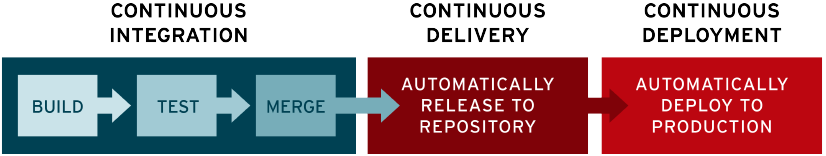
\includegraphics[width=0.85\textwidth]{ci-cd-flow-desktop}
    \caption{\textit{CI/CD} tok}
\end{figure}

Moguće je da \textit{CI/CD} obuhvati povezane prakse kontinualne integracije i kontinualnog dostavljanja, 
ili sve 3 povezane prakse kontinualne integracije, kontinualnog dostavljanja i kontinualnog 
raspoređivanja. Dodatnu komplikaciju stvara to što se kontinualna isporuka može nekada koristiti 
na način koji obuhvata procese kontinualnog raspoređivanja.

%TODO ovoj recenici nije ovde mesto, vec pre opisivanja CI i CD. Isto i za naredni pasus
\textit{CI/CD} je proces, često predstavljen kao tok, koji obuhvata uvođenje visokog stepena 
automatizacije i kontinualnog praćenja razvoja aplikacije.

Od slučaja do slučaja, na šta se termini konkretno odnose zavisi od toga koliko je automatizacije 
ugrađenou \textit{CI/CD} tok. Mnoga preduzeća započinju dodavanjem \textit{CI}, nakon čega uvode automatizaciju 
dostavljanja i raspoređivanja.

\subsection{Kontinualna integracija}
U razvoju modernih aplikacija, cilj je da više programera istovremeno radi na različitim delovima 
aplikacije. Međutim, ukoliko je organizacija postavljena tako da se spajanje koda sa svih grana 
vrši u jednom danu, takav posao može biti monoton, manuelan i dugotrajan. To se dešava u slučajevima 
kada programer vrši izmene na aplikaciji i na taj način povećava šansu za nastajanje konflikta sa 
izmenama koje istovremeno prave drugi programeri.

Kontinualna integracija (\textit{CI}) pomaže programerima da spoje izmene na kodu na deljenu granu češće, 
čak i na dnevnom nivou. Nakon spajanja izmenjenih delova koda, izmene se validiraju tako što se 
automatski gradi aplikacija i pokreće se više nivoa automatskog testiranja. To znači da se testira 
sve, od klasa i funkcija do različitih modula koji su deo aplikacije. Ako automatski testovi pronađu 
konflikt između novog i postojećeg koda, \textit{CI} olakšava rešavanje konflikata.

\subsection{Kontinualno dostavljanje}
Nakon automatskog građenja aplikacije i testiranja u \textit{CI}, kontinualno dostavljanje automatizuje 
puštanje prethodno validiranog koda u repozitorijum. Kako bismo imali efektivan proces kontinualne 
dostave, važno je da imamo već ugrađen \textit{CI} u protoku. Cilj kontinualnog dostavljanja jeste postojanje 
baze koda koja je uvek spremna za raspoređivanje na produkciono okruženje.

U kontinualnom dostavljanju, svaka faza, počevši od spajanja izmenjenog koda do dostavljanja 
verzija spremnih za produkciju, podrazumeva automatsko testiranje i automatizaciju raspoređivanja 
koda. Na kraju tog procesa, operacioni tim je u mogućnosti da brzo i jednostavno rasporedi 
aplikaciju na produkciju.

\subsection{Kontinualno raspoređivanje}
Poslednja faza \textit{CI/CD} protoka je kontinualno raspoređivanje. Kao dodatak kontinualnom dostavljanju, 
koji automatizuje isporuku verzija spremnih za produkciju, kontinualno raspoređivanje automatizuje 
puštanje aplikacije u produkciju. U velikoj meri se oslanja na dobro osmišljeno automatsko testiranje.

U praksi, kontinualno raspoređivanje znači da izmene na aplikaciji mogu biti na produkciji za samo 
nekoliko minuta (pod pretpostavkom da su automatski testovi uspešno završeni).

Sve povezane prakse \textit{CI/CD} čine raspoređivanje aplikacije manje rizičnim, stoga je lakše pustiti 
promene u aplikaciji u delovima, pre nego odjednom.~\cite{CI_CD}

\subsection{GitHub Akcije}
Za verzionisanje koda se može koristiti \textit{GitHub}. Pored verzionisanja, on pruža i alate za automatizaciju 
kontinualne integracije, isporuke i raspoređivanja, kroz alat koji su nazvali \textit{GitHub Akcije} 
(eng. \textit{GitHub Actions}). 
\textit{GitHub Akcije} su zasnovane na događajima, što znači da mogu da pokrenu niz komandi koje će se desiti 
posle navedenog događaja. Na primer, svaki put kada neko napravi \textit{zahtev za promenu} 
(eng. \textit{Pull Request}) u repozitorijumu, može se automatski pokrenuti komanda koja pokreće 
testove. 

\textit{GitHub Akcije} koriste \textit{YAML} fajlove kako bi se definisale komponente toka rada. Ovi fajlovi 
se čuvaju u repozitorijumu, u folderu pod nazivom \mbox{\texttt{.github/workflows}}.

Komponente koje postoje u \textit{GitHub Akcijama} su: 

\begin{itemize}
    \item Tok rada (eng. \textit{Workflow})
    \item Događaj (eng. \textit{Event})
    \item Posao (eng. \textit{Job})
    \item Korak (eng. \textit{Step})
    \item Akcija (eng. \textit{Action})
    \item Izvršilac (eng. \textit{Runner})
\end{itemize}

\begin{figure}[h]
    \centering
    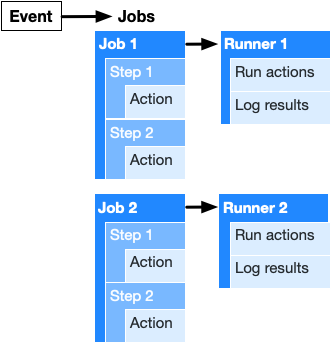
\includegraphics[width=0.5\textwidth]{overview-actions-design}
    \caption{Prikaz interakcija komponenata \textit{GitHub Akcija}}
\end{figure}

\subsubsection{Tok rada}
Tok rada je automatizovana procedura koja se definiše u repozitorijumu. Tokovi rada su sastavljeni 
od jednog ili više poslova i mogu se pokrenuti na određeni događaj ili biti zakazani u određeno vreme. 
Tok rada se može koristiti da se aplikacija izgradi, testira, spakuje, isporuči ili rasporedi na 
različita okruženja.

\subsubsection{Događaji}
Događaj je specifična aktivnost koja pokreće tok rada. Na primer, aktivnost može nastati kad neko napravi 
zahtev za promenu. Aktivnost ne mora da bude u okviru \textit{GitHub}-a. Ona može da predstavlja i poziv od strane 
nekog eksternog sistema.

\subsubsection{Posao}
Posao predstavlja skup koraka koji treba da se izvrše %TODO nad istim izvrsiocem
nad istim izvršiocem. Tok rada sa više poslova 
će pokrenuti ove poslove u paraleli. Naravno, tok rada se može podesiti tako da izvršava poslove 
sekvencijalno. Na primer, tok rada može imati dva sekvencijalna posla koji izgrađuju i testiraju kod, 
gde je posao za testiranje zavisan od toga da li kod uopšte može da se izgradi. Ako posao za izgradnju 
ne uspe, posao za testiranje se neće ni pokretati.

\subsubsection{Korak}
Korak predstavlja jedan zadatak koji može pokrenuti komandu unutar posla. Korak može biti ili akcija ili 
komandni skript. Svaki korak unutar posla se izvršava nad istim izvršiocem, što dozvoljava akcijama da 
dele podatke između sebe.

\subsubsection{Akcija}
Akcije predstavljaju samostalne komande koje se mogu kombinovati u korake kako bi sačinile jedan posao.
Akcije su najmanje portabilne jedinice građe toka rada. Korisnici mogu sami da naprave svoje akcije,
ili da koriste akcije koje su napravljene od strane \textit{GitHub} zajednice. 

\subsubsection{Izvršilac}
Izvršilac je mašina nad kojom se \textit{GitHub Akcije} izvršavaju. Izvršilac osluškuje pokrenute poslove,
pokreće jedan posao za drugim, i šalje izveštaje \textit{GitHub}-u o napretku, logovima i rezultatima. Ove 
mašine mogu da budu bazirane na \textit{Linux}, \textit{Windows} i \textit{macOS} operativnim sistemima, a svaki posao 
unutar toka rada se pokreće iz novog virtualnog okruženja.~\cite{GitHubActions}
